\documentclass[11pt]{article}

\usepackage[UTF8]{ctex} % for Chinese 

\usepackage{setspace}
\usepackage[colorlinks,linkcolor=blue,anchorcolor=red,citecolor=black]{hyperref}
\usepackage{lineno}
\usepackage{booktabs}
\usepackage{graphicx}
\usepackage{float}
\usepackage{floatrow}
\usepackage{subfigure}
\usepackage{caption}
\usepackage{subcaption}
\usepackage{geometry}
\usepackage{multirow}
\usepackage{longtable}
\usepackage{lscape}
\usepackage{booktabs}
\usepackage{natbib}
\usepackage{natbibspacing}
\usepackage[toc,page]{appendix}
\usepackage{makecell}

\title{孟子}
\date{}

\linespread{1.5}
\geometry{left=2cm,right=2cm,top=2cm,bottom=2cm}

\begin{document}

  \maketitle
  
  \begin{figure}[H]
    \centering
    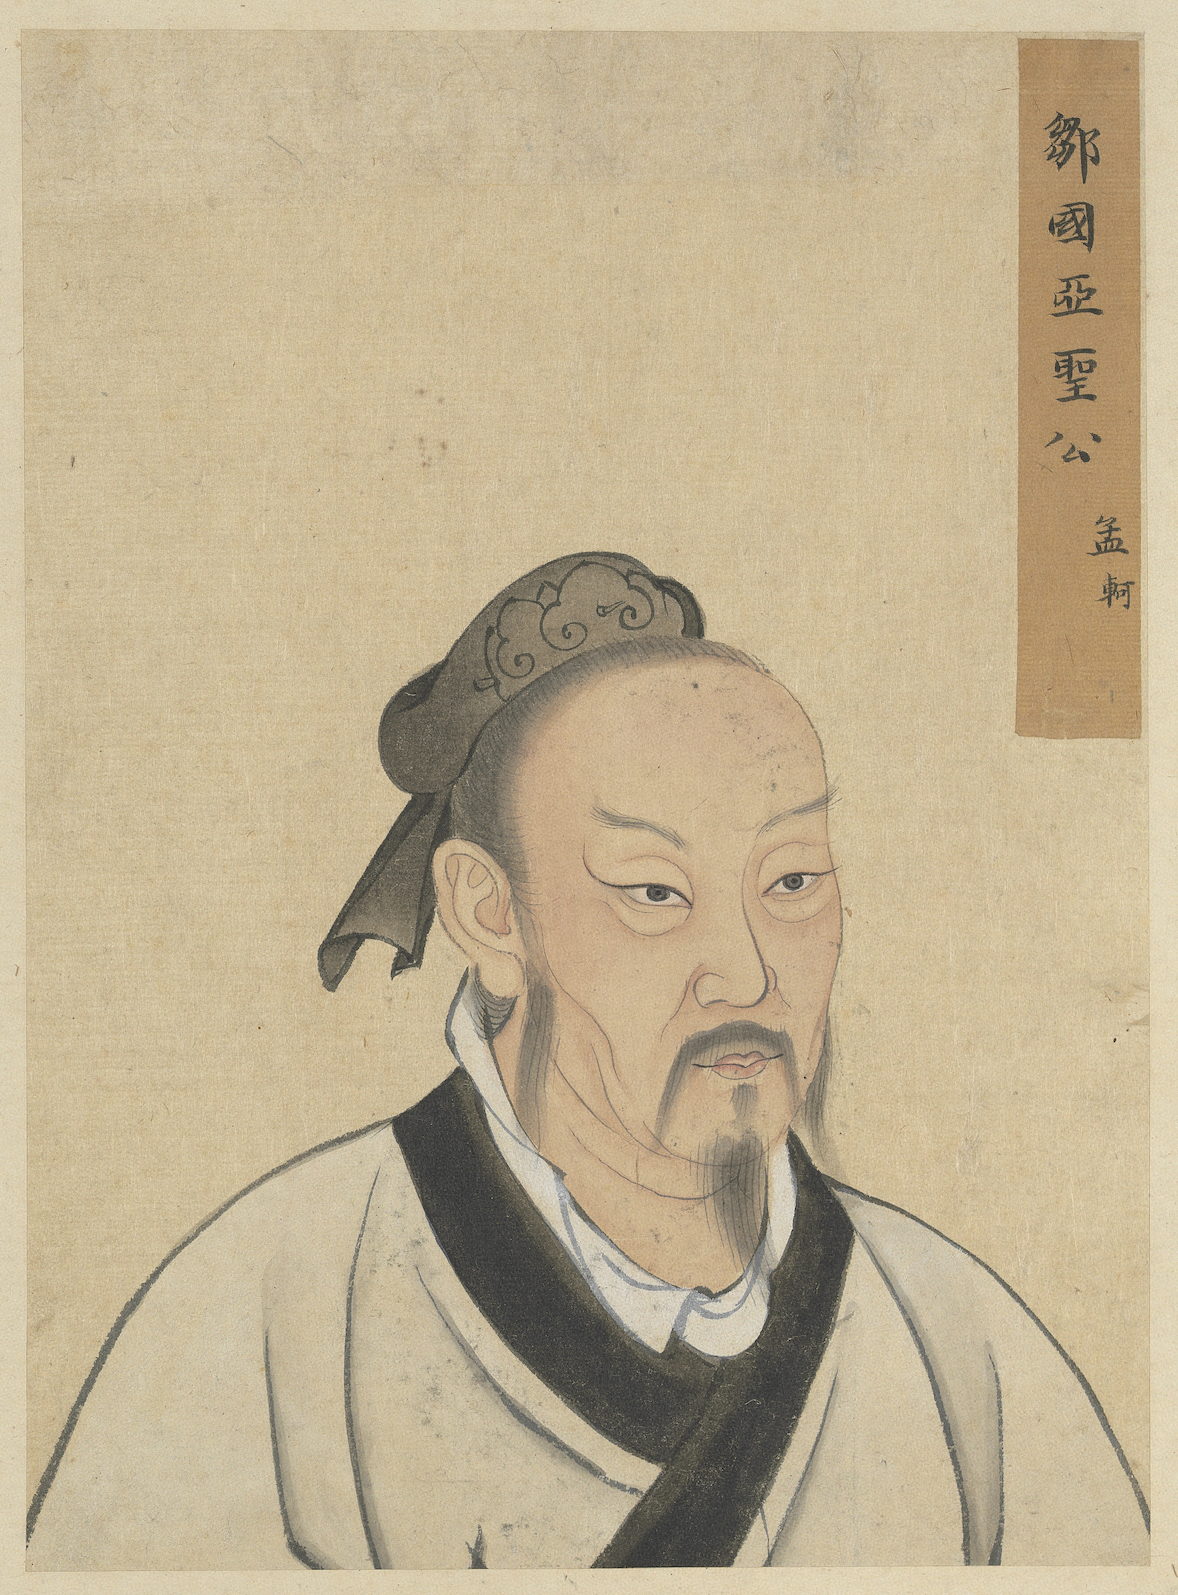
\includegraphics[width=0.7\textwidth]{../Figures/MengZi.jpg}
    \caption{孟子像。台湾国立故宫博物院藏。}
  \end{figure}

  \newpage
  
  \linenumbers

孟子(372 BC-289 BC),名轲,表字无传。
今之所谓孟子字子舆、子居、子车等,皆出自魏晋之后,当系后人附会。
大抵孟子为继孔子之后能发展其理论学说者,系儒家一甚大人物,却无表字,实在令人难以接受,故强为之字。

\newline

孟子生于百家争鸣之盛时。
彼时杨朱、墨翟已为显学,而慎宋之流,仪秦之徒,亦各肆其说。
孟子以继承孔子之学自居,致力于捍卫儒学,驳斥诸家之说,以“正人心、息邪说、距诐行、放淫辞”为己任,其文雄辩滔滔、气势不俗,颇值一观。

\newline

孔子之学,以人之自觉作为价值判断之根源,由此衍生“仁”(公心)、“义”(正当)、“礼”(秩序)之脉络,最终落于政治实践。
孟子对孔子理论之发展,主要体现于孔子理论脉络的两端。
其一是人之自觉如何得以完成价值之判断?
孔子对此未有一明确答复。
孟子则以价值判断为人之一固有属性。
其二系政权转移问题。
各人皆有各人之权利义务。
倘某人侵犯他人之权利,或未完成自身之义务,则可由政府,或者说统治者以国家权力加以制裁。
但若统治者未能完成自身之义务,或侵犯他人之权利,是否应该加以制裁?
由谁来制裁?
如何制裁?
换言之,如何处理“君不君”的情况?
孔子对此未有涉及。这一问题,亦留待孟子加以解答。
  
\section{性本善}
“性”指人之自觉主宰,“本”指本质,“善”指价值意识。
所谓“性本善”,是说人之价值意识为自觉心之本有,或为自觉心之固有本质。
人于生活中,对各种行为、主张,皆有其应当或不应当、合理或不合理之自觉。
对某种已有之事像,若觉其不应当,即有割离排斥之自觉。
此种判断出自人之自觉,独立于利害考虑之外。
换言之,人可以不由于利害或自身感受等原因,而仍自觉事务之应当或不应当。
此种价值意识,为人自觉心之固有属性,通过不同形式得以表现,成为各种德性之根源。
即人之自觉为各种德性之种子。
欲使各德性圆满展开,需人自觉之努力。
《孟子·公孙丑上》以孺子将入于井加以说明:

\textit{所以谓人皆有不忍人之心者:今人乍见孺子将入于井,皆有怵惕恻隐之心。非所以内交于孺子之父母也,非所以要誉于乡党朋友也,非恶其声而然也。由是观之,无恻隐之心,非人也;无羞恶之心,非人也;无辞让之心,非人也;无是非之心,非人也。恻隐之心,仁之端也;羞恶之心,义之端也;辞让之心,礼之端也;是非之心,智之端也。人之有是四端也,犹其有四体也。有是四端而自谓不能者,自贼者也;谓其君不能者,贼其君者也。凡有四端于我者,知皆扩而充之矣,若火之始然,泉之始达。苟能充之,足以保四海;苟不充之,不足以事父母。”}

所谓“不忍人之心”,指人之价值自觉。
由于此自觉心,人“乍见孺子将入于井”时,皆有此事件为不应当之自觉,遂有排斥之心,故能“怵惕恻隐”。
这种排斥不合理事件之自觉与个人之利害无关。
由此种价值自觉生“恻隐”“羞恶”“辞让”“是非”诸心,为仁义礼智诸德之种子。
“扩而充之”指诸德之展开所需之自觉努力。

\section{取义去利}
人之自觉心本有价值判断之能力。
换言之,人天生即有仁义之心。
既然如此,又何以有君子小人之分别?
“钧是人也,或为大人,或为小人,何也?”答曰:或从义也,或从利也;从义者为大人,从利者为小人。

\newline

所谓利,系人之感官需求,或者说是趋利避害之生物本能,为人生而具有之欲望。
利不具有普遍性,所谓各人心机各自谋。
利具有特殊性,每个人的利不尽相同,甚至互相冲突。
若以利作为价值规范之基础,则必生混乱。
《孟子·梁惠王上》载:

\textit{孟子见梁惠王。王曰:“叟不远千里而来,亦将有以利吾国乎?”孟子对曰:“王何必曰利?亦有仁义而已矣。王曰’何以利吾国’?大夫曰’何以利吾家’?士庶人曰’何以利吾身’?上下交征利而国危矣。万乘之国弑其君者,必千乘之家;千乘之国弑其君者,必百乘之家。万取千焉,千取百焉,不为不多矣。苟为后义而先利,不夺不餍。未有仁而遗其亲者也,未有义而后其君者也。王亦曰仁义而已矣,何必曰利?”}

此处谓王、大夫、士庶人皆一味追求私利,彼此冲突,生“不夺不餍”之混乱。

\newline

所谓义,乃人本有判断正当与不正当之自觉能力,系普遍性真理,无个体之差异。
故以义判断事物,以本有之价值自觉为方向,方为“大人”。
《孟子·告子上》载:

\textit{口之于味也,有同耆焉;耳之于声也,有同听焉;目之于色也,有同美焉。至于心,独无所同然乎?心之所同然者何也?谓理也,义也。圣人先得我心之所同然耳。故理义之悦我心,犹刍豢之悦我口。”}

此处谓人之自觉心求义,一如感官要求其满足。

\newline

换言之,所谓利、义,均为人生而具有之性质。
利追求个体物质欲望之满足,个体差异显著,不能为价值判断之标准;义追求正当并否定不正当,系普遍真理,应成为价值判断之标准。
  
\section{养气成德}
综上所述,人本有判断正当与不正当之自觉,即从义之自觉;亦有趋利避害、追求感官满足之欲望,即逐利之本能。
就理论意义而言,从义还是逐利,由人之自主所决定,其主宰权在于人自身。
君子人自当从义而终。
然而在实践中,义和利多有种种混杂纠结,遂生迷乱。
换言之,从义实系一“应当性”问题,而非“必然性”问题。
由此,本节所论之问题为如何才能从义而终?
如何才能在实践中坚持发挥价值自觉之功效?
答曰:养气。

\newline

所谓气,指人之生命力和生命感,系人之情感和本能所产生的冲动。
养气,即将情感冲动理性化,将其置于人之价值自觉之统帅之下。
换言之,人之冲动,可由利所驱动,亦可由义所驱动。
利具有特殊性,不足以作为此类冲动之依据,否则必生迷乱。
而义为普遍真理,系生命冲动之坚实根基。
此种价值自觉所统帅的生命力量浩然无际,至大至刚。
《孟子·公孙丑上》载:

\textit{敢问何谓浩然之气?曰:难言也。其为气也,至大至刚,以直养而无害,则塞于天地之间。其为气也,配义与道;无是,馁也。}

《孟子·公孙丑上》引曾子之言:

\textit{自反而不缩,虽褐宽博,吾不惴焉?自反而缩,虽千万人,吾往矣。}

  
\section{民为贵}
至此,孟子之心性理论已基本得立。
孟子谓价值自觉,即义,为人之固有属性,亦是普遍真理。
人需以普遍性的义统帅生命情意,而不是以特殊性的利为其根基。
现论孟子之政治思想,自民贵始。

\newline

民为邦本的观念在中国起源甚早。
《尚书·皋陶谟》载:
  
\textit{天聪明,自我民聪明;天明威,自我民明威。}

引文中所谓“天”,系一至高主宰,犹今之宗教所言上帝者。
然此至高之“明”、“威”均出自民。
换言之,至高主宰之意志需假借人民群众来表达,民为天之代表。

\newline

孟子则直接肯定民之重要性。
《孟子·尽心下》载:

\textit{民为贵,社稷次之,君为轻。}

更进一步,孟子直接将政权之得失归诸民意,弗言天意。

《孟子·离娄上》载:

\textit{桀纣之失天下也,失其民也;失其民者,失其心也。得天下有道:得其民,斯得天下矣 。得其民有道:得其心,斯得民矣。}

如此,政权之转移由民心向背决定。
统治者失去民心,自然也就要失去政权。
换言之,君不君,便无君。

《孟子·梁惠王下》载:
  
\textit{孟子谓齐宣王曰:“王之臣有托其妻子于其友,而之楚游者。比其反也,则冻馁其妻子,则如之何?”王曰:“弃之。”曰:“士师不能治士,则如之何?”王曰:“已之。”曰:“四境之内不治,则如之何?”王顾左右而言他。}

此节虽不明言,但其中之暗示甚为明显,且行文颇值得玩味。
臣之友未能完成委托,使妻子冻馁,此不足为友,故与之绝交;士师无法管理手下,未能完成官员之义务,此不足为官,故罢免之。
一言以蔽之,友人和士师均未能完成应尽之责任,故剥夺其友人和士师之身份。
则如君王何?
身为君王,不能治理国家,完不成其应尽之责任,应当如何处置?
依前例,自然是要剥夺其君王之身份。
齐宣王“顾左右而言他”,足见其心虚。
可以想见孟子步步设坑之蔫坏损,以及齐王无话可答之窘迫。
实在想象不出来的话,建议参考刘宝瑞相声《官场斗》中刘墉参乾隆偷坟掘墓那一段。

\newline

更进一步,如何制裁不君之君?
此系政权转移之实践问题,由孟子盛赞汤武革命,可窥见其观点。
《孟子·梁惠王下》载:

\textit{齐宣王问曰:“汤放桀,武王伐纣,有诸?”孟子对曰:“于传有之。”曰:“臣弑其君,可乎?”曰:“贼仁者谓之贼,贼义者谓之残,残贼之人谓之一夫。闻诛一夫纣矣,未闻弑君也。”}

按古之春秋笔法,下杀上曰“弑”,杀有罪为“诛”。
“弑君”系遗臭万年之大恶。
齐宣王谓汤伐夏、武伐商为“弑”,言其身为臣民而反叛君主。
孟子则称之为“诛”,言桀纣身为君王,弗行君道,失去民心,即为有罪。
臣民诛之,非弑君也。
换言之,现有政权如未能完成其义务,则民可将其推翻,另立一新政权。
新政权之得立,其根本原因在于得民心,在于赢得人民拥护。
  
\section{王道}
既然民心向背为政权得失之根本原因,则现有政府应当如何赢得人民拥护?
答曰行王道。
所谓王道,实指一套具体措施,以提高人民之生活水平。
《孟子·梁惠王上》有详细描述孟子理想中的王道:
  
\textit{不违农时,谷不可胜食也;数罟不入洿池,鱼鳖不可胜食也;斧斤以时入山林,材木不可胜用也。谷与鱼鳖不可胜食,材木不可胜用,是使民养生丧死无憾也。养生丧死无憾,王道之始也。五亩之宅,树之以桑,五十者可以衣帛矣;鸡豚狗彘之畜,无失其时,七十者可以食肉矣;百亩之田,勿夺其时,数口之家可以无饥矣;谨庠序之教,申之以孝悌之义,颁白者不负戴于道路矣。七十者衣帛食肉,黎民不饥不寒,然而不王者,未之有也。}

可见,孟子之王道,实为其民贵思想之延伸,其旨在于使民安乐。
孟子以为,行此王道,使民众安乐,遂能赢得人民拥护。能得民心则必可王也。

\newline

更进一步,王道之实行,依赖于掌权者本身能立仁心,施仁政。
《孟子·梁惠王上》载:

\textit{梁惠王曰:“晋国,天下莫强焉,叟之所知也。及寡人之身,东败于齐,长子死焉;西丧地于秦七百里;南辱于楚。寡人耻之,愿比死者一洒之,如之何则可?”孟子对曰;“地方百里而可以王。王如施仁政于民,省刑罚,薄税敛,深耕易耨;壮者以暇日修其孝悌忠信,入以事其父兄,出以事其长上。可使制梃以达秦楚之坚甲利兵矣。彼夺其民时,使不得耕耨以养其父母。父母冻饿,兄弟妻子离散,彼陷溺其民,王往而征之,夫谁与王敌?故曰:‘仁者无敌。’王请勿疑。”}

执政者需先立仁心,有存公去私之境界,为人着想之自觉,方能在政治实践中以民为重,推行王道。此即所谓“先王有不忍人之心,斯有不忍人之政”。可见,孟子之政治理想以“有德者执政”为中心,言王道之实行依赖于统治者之德性。后世所谓君圣臣贤,即是此理。
  
\section{社会分工}
至此,孟子理论之主体部分已论述完毕。
孟子思想之主题包括心性理论和政治理论。
心性理论以性善为中心,区分义利,终于养气从义之实践功夫。
政治理论以民本为核心,提倡仁政,最终落于统治者之道德自觉。
除此两部分之外,孟子仍有论述其他问题,颇有理论意义,但仅透露出部分观点,缺乏较为系统之陈述。
现撮其大意,以为补充。
先论孟子社会分工之观念,进一步延伸可明知识分子之社会地位。

\newline

孟子论社会分工,见诸《孟子·滕文公上》:

\textit{有为神农之言者许行,自楚之滕,踵门而告文公曰:“远方之人闻君行仁政,愿受一廛而为氓。”文公与之处。其徒数十人,皆衣褐,捆屦、织席以为食。陈良之徒陈相与其弟辛,负耒耜而自宋之滕,曰:“闻君行圣人之政,是亦圣人也,愿为圣人氓。”陈相见许行而大悦,尽弃其学而学焉。陈相见孟子,道许行之言曰:“滕君则诚贤君也,虽然,未闻道也。贤者与民并耕而食,饔飧而治。今也滕有仓禀府库,则是厉民而以自养也,恶得贤?”
孟子曰:“许子必种粟而后食乎?”曰:“然。”“许子必织布然后衣乎?”曰:“否,许子衣褐。”“许子冠乎?”曰:“冠。”曰:“奚冠?”曰:“冠素。”曰:“自织之与?”曰:“否,以粟易之。”曰:“许子奚为不自织?”曰:“害于耕。”曰:“许子以釜甑爨,以铁耕乎?”曰:“然。”“自为之与?”曰:“否,以粟易之。”“以粟易械器者,不为厉陶冶;陶冶亦以其械器易粟者,岂为厉农夫哉?且许子何不为陶冶,舍皆取诸其宫中而用之?何为纷纷然与百工交易?何许子之不惮烦?”曰:“百工之事固不可耕且为也。”“然则治天下独可耕且为与?有大人之事,有小人之事。且一人之身,而百工之所为备,如必自为而后用之,是率天下而路也。故曰,或劳心,或劳力;劳心者治人,劳力者治于人;治于人者食人,治人者食于人,天下之通义也。“}

许行之说,其大要为人人均需从事农业生产,否则便是剥削他人劳动成果,即“厉民而以自养”。
孟子诘之,谓耕种并非特殊行业。
耕者以粟换购陶铁之器械,陶冶之工匠以其器械换购粟,此系人各执一业,各有其工作成果,互相交换,无所谓剥削。
再者,个人知识、技巧、精力有限,固不能做尽百工之事,可见社会分工之必要。
更进一步,随着社会发展,有不属于直接生产之工作,如管理公共事务、设计制度法律、维护社会秩序等。
此类“劳心”之工作,亦为劳动,且其重要性绝不在“劳力”之下。
由此,知识分子若从事有益于社会大众之非生产性工作,亦是劳动,且较一般生产工作有更高价值。
  
\section{历史观}
现论孟子之历史观,系关于历史演变之看法,以及人之意志、力量于历史进程中有何作用等问题。
孟子承认既成之历史为事实意义之限定,为未来之发展提供一种趋势。
此种趋势在价值上为中立。
客观趋势一旦成立,人之成败便受其限制。
《孟子·离娄上》载:

\textit{孟子曰:“天下有道,小德役大德,小贤役大贤;天下无道,小役大,弱役强。斯二者天也,顺天者存,逆天者亡。”}

此处言“天”,乃就历史发展趋势而论。
“顺天者存,逆天者亡”者,谓人当顺势求存。

\newline

然而,客观之趋势仅为历史演变之限制,而非决定性因素。
孟子坚持人之力量,以人在历史中有最终主宰性之立场。
故《孟子·离娄上》又载:

\textit{今也小国师大国,而耻受命焉;是犹弟子而耻受命于先师也。如耻之,莫若师文王;师文王,大国五年,小国七年,必为政于天下矣。}

此处引“小邦周”取代“大邑商”之历史,强调人之自觉努力可超越已有之趋势。

此一态度实出其政治理论。
既以为统治者立仁心,便可行王道,由此可得王天下之效用,则对人之意志能决定历史演进实已预认矣。
其历史观念则进一步强调人于历史发展中的主宰性。
客观事实固然对人有所限制,但不起决定性作用。


\end{document}